%KOKO
\documentclass[lang=cn]{elegantpaper}

\usepackage{array}
\usepackage{courier}
\usepackage{xcolor}
\usepackage{tabulary}
\usepackage{float}
\usepackage{makecell}
\usepackage{multirow}
\usepackage{zhnumber}

\title{VoIP:原理与协议比较}
\author{于海鑫 \\ 2017211305 班 \\ 2017211240}
\institute{北京邮电大学计算机学院}

\version{}
\date{\zhtoday}


% 本文档命令
\usepackage{array}
\newcommand{\ccr}[1]{\makecell{{\color{#1}\rule{1cm}{1cm}}}}

\begin{document}

\maketitle

\begin{abstract}
    互联网的发展给人们的生活带来了极大的遍历,越来越多的十四通信技术出现在了人们的生活中。 VoIP 就是在这种背景下兴起的新技术,它通过廉价的 Internet 资源,把语音信号以数据包的形式在网络上传输。随着 VoIP 技术的广泛部署,一些安全问题已经出现。本文中我们会介绍 VoIP 技术下比较常用的两类协议:H.323 与 SIP,以及一些支持其运行的协议。最后会对两类协议做一个比较。
    \keywords{VoIP,SIP,H.323}
\end{abstract}

\section{引言}

基于 IP 的语音传输(VoIP)技术\cite{goode2002voice}是一种语音通话技术。其经由互联网来实现语音通话以及多媒体会议,也就是使用互联网来进行语音通信。该技术的非正式名称有 IP 电话、互联网电话、宽带电话等。通常来说,VoIP 技术允许可以访问互联网的任意两个用户进行通话,有些 VoIP 服务的提供商也会允许用户接受/拨打传统座机号码的电话\cite{pershan2005methods},不过这类服务通常会收取费用。在 VoIP 网络内,语音信号会被取样并数字化,之后被压缩转换成 IP 数据包,之后经由传统的 IP 网络进行传输。在 VoIP 技术中比较重要的是信令协议,其作用在于帮助会话双方建立、断开连接,以及协商通话时使用的协议等信息。

近年来,基于 VoIP 技术的通信产品逐渐出现在市面上,今年以来由于疫情的影响更是大规模的开始占领市场。通常来说,VoIP 被广泛部署的主要原因是其成本极低,性价比极高。其他的一些原因可能是:

\begin{itemize}
    \item 传统的语音电话满足不了用户的需求,需要视频等多媒体技术的支持
    \item 传统的语音电话无法使用
\end{itemize}

\subsection{核心问题}

随着 VoIP 技术的广泛应用与部署,一些相关问题已经浮出水面亟待解决。这些问题很多都是继承自 IP 网络的问题,也有一些是厂商不遵循标准导致的问题。以下是我们总结出的 VoIP 技术部署时要注意的几个核心问题:

\subsubsection{服务质量}

这一问题是老生常谈的问题了,任何一个在 IP 网络上构建自己服务的项目都会遇到这一问题。众所周知,IP 网络构建时候只是提供了一种尽力而为的服务,没有实时性的保障,也没有一定送达的承诺。语音交流服务十分注重实时性,一旦延迟在某个阈值之上,用户的体验将大打折扣。为了解决服务质量的问题,一些在 IP 网络上进行优化的技术也被频繁的用在了 VoIP 实现上,比如错误纠正,即通过纠错码技术对发生传输错误的包进行纠正,而不是直接丢弃,以及优先发包,即调高与 VoIP 相关的 IP 包的优先级。

\subsubsection{互操作性}
在互联网上,关于 VoIP 的服务端、客户端的实现都非常多。不同厂家的产品可能难以互相通信,以此减少了这一技术的诱人程度。为了达成互操作的可能性,通信协议出现了。目前最常见的 VoIP 技术的信令协议为 H.323 以及 SIP,分别从电话通信与互联网通信的角度定义了 VoIP 的协议。我们将在后续两个章节分别讲述这两类协议。

\subsubsection{安全性}
互联网是开放的,也就是说其实任何人都可能在通信链路上抓到你的包,此时就会产生一些安全问题。比如与公司重大战略相关的消息肯定不想被第三方用过抓包的方式偷听到。为了解决这一问题,最常见的方式就是使用加密技术或者隧道技术。在 VoIP 技术中,最常见的解决安全问题的技术分别为隧道技术以及 SSL 技术。

\subsection{与传统电话网络的交互}
尽管互联网已经大规模普及,但是仍存在只能访问传统电话网络但是无法连接数据的情况。我们需要提出一种将 VoIP 网路与传统电话交换机网络无缝互操作的方式。

\section{H.323 协议}

H.323\cite{hersent_ip_2000} 协议由 ITU-T 组织拟定,该协议为任何数据包网络多媒体会话提供支持。大量应用程序都基于这一协议实现,最出名的包括 GNU Gatekeeper 计划等。H.323 是 ITU-T 的 H.32x 协议系列的一部分。这一系列的协议,也尝试解决多媒体通信综合业务数字网(ISDN)及公共交换电话网络(PSTN)或信号系统 7(SS7)和 3G 移动网络的通信问题问题。

尽管 H.323 协议最初是专门为多媒体通信技术定义的,但是现在最主要用在 IP 网络电话系统。H.323 协议适用范围包括数据、视频和语音及其融合多媒体通信,支持语音通信为必备功能,而视频和数据通信是可选功能。H.323 适用的 IP 网络是基于分组的网络,如 WAN, Internet 以及 LAN 等。

\subsection{H.323 组成部件}

H.323定义了四个逻辑组件,即终端,网关,网守和多点控制单元(MCU)。其中终端,网关和MCU被称为端点。下面将分别介绍这几类组件:

\subsubsection{终端}
终端是提供实时双工的 LAN 客户端。所有的 H.323 终端都必须支持 H.245,Q.931,RAS 协议以及 RTP 协议。其中H.245用于准许信道的使用,Q.931 用于处理呼叫信令和建立呼叫,RTP是实时传输协议,RAS 则是用于与网守交互时承载语音数据包的协议。

当然,终端也可能支持与视频会议相关的协议,这些不是本文的重点,我们掠过。

\subsubsection{网关}
网关设备的主要作用是处理和其他协议的翻译和互通,即他们执行不同传输格式之间的翻译,例如 H.225 到 H.221 之间的转换。 它们还能够在音频和视频编解码器之间转换。网关也是 PSTN 网络到 VoIP 网络的接口。其可以接收来自于传统公共电话网络的语音辛哈,并将之转换为 H.323 终端可以理解的信号。

对于 H.323 来说,网关设备是可选的。例如当整个网络都构建在局域网内,且没有别的要求时,我们就没有必要加一个网关,因为整个网络都可以直接互相通信。

\subsubsection{网守}

网守是在为H.323终端、网关和MCU提供服务例如地址转换和网络访问控制的网络的一个H.323实体。并且,它们还能提供带宽管理、记帐和拨号方案等其他服务,您可以集中这些服务以提供易卖性。

网守在逻辑上与 H.323 端点(如终端和网关)分离。它们在 H.323 网络中是可选的。但是,如果存在网守,则端点必须使用其提供的服务。
一般来说,网守必须提供以下功能:
\begin{itemize}
    \item \textbf{地址转换}\ 将 H.323 ID(如 gwy1@domain.com)和 E.164 编号(标准电话号码)转换为端点 IP 地址。
    \item \textbf{准入控制}\ 控制是否准许端点进入 H.323 网络。
    \item \textbf{带宽控制}\ 终端带宽需求的管理。
    \item \textbf{区域管理}\ 网守为所有注册的终端提供区域管理在区域,例如,终端注册过程的控制。
\end{itemize}

\subsubsection{MCU}
MCU 主要负责管理多点会议,由必须的多点控制器(MC)和可选的
多点处理器(MP)构成。其通过使用 H.245 协议确定终端的大部分功能,但是数据的多路化是由 MP 进行控制。

\subsection{H.323 协议栈}

下图展示了 H.323 协议族中大部分协议的作用,通常来说一个实现不需要包含全部的协议。我们能够注意到,音频、视频和注册数据包使用UDP进行传输,而数据和控制应用程序包则使用 TCP 作为传输协议。因为篇幅原因,我们暂且略去其具体的解说。

\begin{figure}[H]
    \centering
    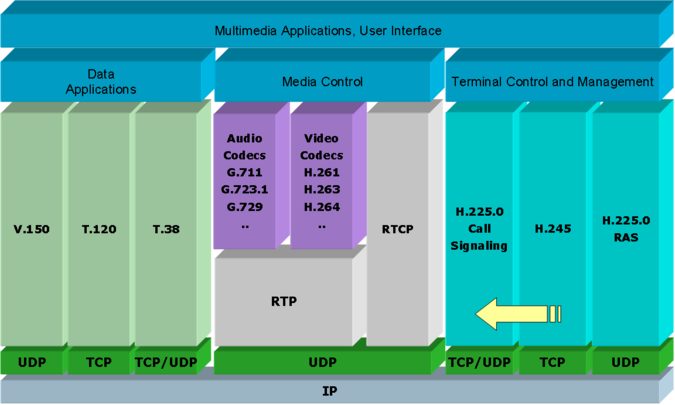
\includegraphics[width=\textwidth]{1}
    \caption{H.323 协议栈 Ref: Wikipedia}
    \label{fig:stack}
\end{figure}

\section{SIP 协议}

SIP 协议\cite{rfc2543}是由 IETF 主导的 VoIP 的标准,其用于创建、修改、结束具有多个参与者的会话,为了提供电话业务它还可以结合不同的标准和协议:特别是需要确保传输(RTP),与当前电话网络的信令互连,能够确保语音质量(RSVP),能够提供目录(LDAP),能够鉴权用户(RADIUS)等等。 SIP 的架构与 HTTP 类似,都是客户端-服务端的架构。客户端生成请求,并发送到服务端。服务端处理请求并把想用发送回客户端。一对请求-回复构成了一个事务。 SI 定义了 INVITE 消息以及 ACK 消息,以此实现了可以通过不可靠通道构建传递呼叫控制信息的可靠通道的过程。 SIP 对于其基础传输协议并未做过多假设,协议自身对可靠性做了保障,不依赖于 TCP 提供的可靠通道。SIP 使用会话描述协议(SDP)进行语音编码器/解码器的协商与识别。SIP 以此描述会话需求,使得通话双方选择一种兼容的媒体类型进行通话。除此之外,其还可以通过代理将请求重定向到别的位置,以此支持一些便利的操作。

SIP 协议主要提供了如下功能:
\begin{itemize}
    \item 名字翻译和用户定位:无论被呼叫方在哪里都确保呼叫达到被叫方。执行任何描述信息到定位信息的映射。确保呼叫(会话)的本质细节被支持。
    \item 特征协商:它允许与呼叫有关的组(这可以是多方呼叫)在支持的特征上达成一致。例如视频可以或不可以被支持。总之,存在很多需要协商的范围。
    \item 呼叫参与者管理:呼叫中参与者能够引入其它用户加入呼叫或取消到其它用户的连接。此外,用户可以被转移或置为呼叫保持。
    \item 呼叫特征改变:用户应该能够改变呼叫过程中的呼叫特征。例如,一呼叫可以被设置为“voice-only”,但是在呼叫过程中,用户可以中途开启视频功能。也就是说一个加入呼叫的第三方为了加入该呼叫可以开启不同的特征。
\end{itemize}


\subsection{SIP 网络要素}

SIP中有两个要素。SIP用户代理和SIP网络服务器。用户代理是呼叫的终端系统元素,而SIP服务器是处理与多个呼叫相关联信令的网络设备。

\subsubsection{用户代理}
用户代理本身具有一客户机元素(用户代理客户机UAC)和一服务器元素(用户代理服务器UAS)。客户机元素初始呼叫而服务器元素应答呼叫。这允许点到点的呼叫通过客户机-服务器协议来完成。

\subsubsection{服务器}

SIP服务器元素提供多种类型的服务器。有三种服务器形式存在于网络中, 分别为
\begin{itemize}
    \item SIP注册服务器
    \item SIP代理服务器
    \item SIP重定向服务器
\end{itemize}
由于呼叫者未必知道被呼叫方的IP地址或主机名,SIP服务器需要能够提供名字解析和用户定位。可以获得的是email形式的地址或与被呼叫方关联的电话号码。使用该信息,呼叫者的用户代理能够确定特定服务器来解析地址信息。

SIP代理服务器接收请求,决定将这些请求传送到何处,并且将它们传送到下一服务器(使用下一跳路由原理)。在网络中可以有多跳。
有状态和无状态代理服务器的区别是有状态代理服务器记住它接收的入请求,以及回送的响应和它转送的出请求。无状态代理服务器一旦转送请求后就忘记所有的信息。这允许有状态代理服务器生成请求以并行地尝试多个可能的用户位置并且送回最好的响应。无状态代理服务器可能是最快的,并且是SIP结构的骨干。有状态代理服务器可能是离用户代理最近的本地设备,它控制用户域并且是应用服务的主要平台。

重定向服务器接收请求,但不将这些请求传递给下一服务器而是向呼叫者发送响应以指示被呼叫用户的地址。这使得呼叫者可以直接联系在下一服务器上被呼叫方的地址。

\subsubsection{SIP 消息类型}
SIP定义了很多消息类型,用于客户端和服务器之间的通信。 这些消息类型为:

\begin{itemize}
    \item INVITE:邀请用户加入通话
    \item BYE:用于终止两个端点之间的连接
    \item ACK:用于确认消息收到
    \item OPTIONS:用于获取有关呼叫选项的信息
    \item REGISTER:将有关用户地址的信息提供给SIP注册服务器
    \item CANCEL:用于终止用户搜索
\end{itemize}

\subsection{SIP 操作概览}

在 SIP 协议中呼叫者和被叫者通过SIP地址标识。 进行SIP呼叫时,呼叫者首先需要找到对应的服务器并向其发送请求。 呼叫者可以直接与被呼叫者联系,也可以通过重定向服务器间接联系。SIP消息标题中的“呼叫ID”字段唯一标识了一次会话。以下是 SIP 协议工作流程的简要描述。

\subsubsection{用户注册}
注册流程图如下:
\begin{figure}[H]
    \centering
    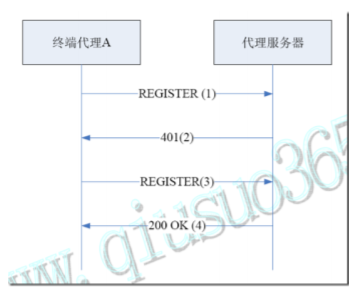
\includegraphics[width=0.5\textwidth]{11}
    \caption{注册流程图}
    \label{fig:register}
\end{figure}
具体流程为:
\begin{enumerate}
    \item 终端向服务器发起 REGISTER 请求
    \item 服务器返回 401,要求进行安全认证
    \item 服务端按照要求加密用户信息,重新 REGISTER
    \item 服务器进行认证,返回 200
\end{enumerate}

\subsubsection{发起通话}
其具体流程为:
\begin{figure}[H]
    \centering
    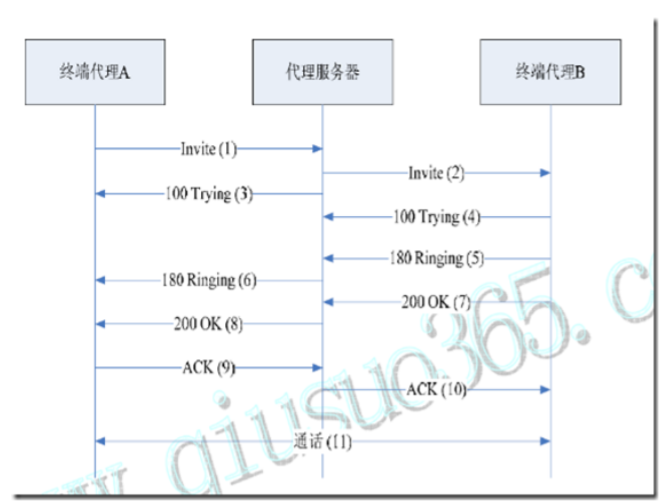
\includegraphics[width=0.8\textwidth]{12}
    \caption{发起通话流程图}
    \label{fig:new}
\end{figure}
各个流程发包如下:

\paragraph{A 用户视角}
\begin{figure}[H]
    \centering
    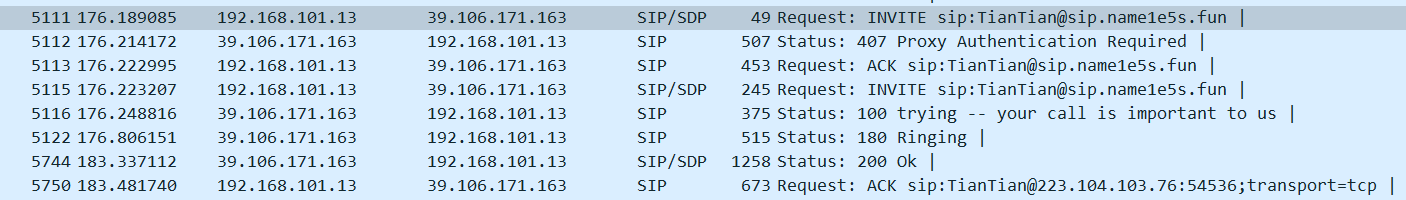
\includegraphics[width=\textwidth]{13}
    \caption{A用户发起通话抓包}
    \label{fig:new}
\end{figure}
\begin{enumerate}
    \item 发起 INVITE 信息
          INVITE 信息中包含了本次通话的详细信息,可以描述通话的具体协议等内容。
    \item 服务端回复 TRYING
    \item 服务端回复 RINGING,此时对面开始响铃
    \item 服务端回复 OK,此时对面接电话
    \item 回应 ACK,我们确定已经接收到了消息。
\end{enumerate}

\paragraph{B 用户视角}
\begin{figure}[H]
    \centering
    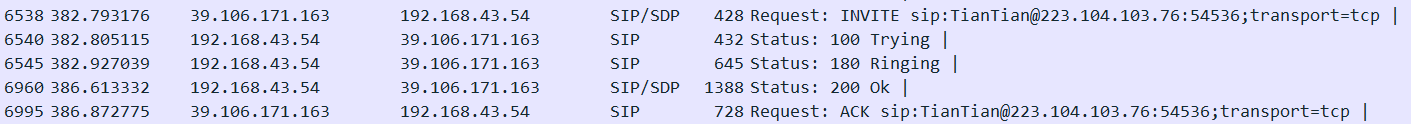
\includegraphics[width=\textwidth]{14}
    \caption{B用户发起通话抓包}
    \label{fig:newB}
\end{figure}
\begin{enumerate}
    \item 收到 INVITE 信息
          此时,我们收到了A发来的INVITE请求,包含了与A相同的通话信息。
    \item 回复 TRYING
    \item 回复 RINGING,标识我们开始响铃
    \item 回复 OK,此时我们接电话
    \item 接收 ACK,我们确定对面已经接收到了消息。
\end{enumerate}

\subsection{结束通话}
其具体流程为:
\begin{figure}[H]
    \centering
    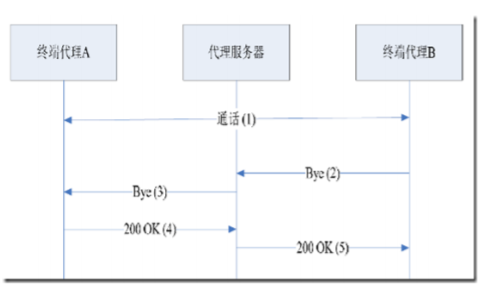
\includegraphics[width=0.8\textwidth]{15}
    \caption{结束通话流程图}
    \label{fig:end}
\end{figure}
其行为较简单,我们不再描述。

\section{支撑协议}

SIP、H.263 系列协议主要是作为信令协议存在,为了实现通话, 其还要与一些协议共同工作,下面我们选择两个相关的支撑协议进行简要介绍。

\subsection{RTP/RTCP}
RTP\cite{rfc1889}是针对Internet上多媒体数据流的一个传输协议, 由IETF作为RFC1889发布,在 VoIP 中常作为语音的传输协议存在。RTP被定义为在一对一或一对多的传输情况下工作,其目的是提供时间信息和实现流同步。RTP的典型应用建立在UDP上,但也可以在TCP或ATM等其他协议之上工作。RTP本身只保证实时数据的传输,并不能为按顺序传送数据包提供可靠的传送机制,也不提供流量控制或拥塞控制,它依靠RTCP提供这些服务。

RTP 主要包括如下功能:
\begin{itemize}
    \item 序列化:RTP数据包中的序列号可以用于检测丢失的数据包
    \item 识别有效负载:在网络内,通常需要动态修改编码以事嘤环境,为此每个 RTP 数据包都会说明其使用的编码
    \item 帧指示:视频/音频通常会以帧为逻辑单元进行发送,RTP 可以为此做出标识
    \item 来源标识:多人会议时,标识参与者是必须的
\end{itemize}

RTCP是一种控制协议,可与RTP一起使用。 在RTP会话中,参与者定期发送RTCP 数据包以获取有关QoS等的有用信息。RTCP提供的主要功能为:
\begin{itemize}
    \item QoS反馈:RTCP可以报告服务质量。 提供的信息包括丢失的数据包数量,往返时间,抖动,这些信息可以用于调整 RTP 的传输速率
    \item 会话控制:通过使用BYE数据包,RTCP允许参与者表明他们将要离开会话
    \item 会话标识:RTCP 中包含用户的个人信息,以此可以区分其他用户的身份
    \item 跨媒体同步:视频和音频通常通过不同的流发送,但是我们通常需要使它们在接收端是同步的,防止出现不对应。 RTCP提供了流同步所需的信息
\end{itemize}

\subsection{RTSP}
RTSP(Real Time Streaming Protocol)\cite{rfc2326}是由Real Network和Netscape共同提出的如何有效地在IP网络上传输流媒体数据的应用层协议。RTSP对流媒体提供了诸如暂停,快进等控制,而它本身并不传输数据,RTSP的作用相当于流媒体服务器的远程控制。服务器端可以自行选择使用TCP或UDP来传送串流内容,它的语法和运作跟HTTP 1.1类似,但并不特别强调时间同步,所以比较能容忍网络延迟。RTSP 主要提供了如下功能:
\begin{itemize}
    \item 从服务器获取媒体:RTSP 客户端可以请求服务端发送数据
    \item 邀请媒体服务器参加会议:可以邀请媒体服务器参加会议播放媒体或录制演示文稿
\end{itemize}

\subsection{SDP}
SDP\cite{rfc2327}主要用于两个会话实体之间的媒体协商。其包含如下信息:
\begin{itemize}
    \item 会话名称、会话目的
    \item 会话地址、端口号
    \item 开始时间、结束时间
    \item 接收媒体的方式
    \item 会话带宽
    \item 会话联系人
\end{itemize}

以上消息以简单的文字形式发送。当使用 INVITE 信息初始化一次 SIP 会话时,其内部就会包含一个 SDP 包,以此实现双方的协商。

\section{H.263 与 SIP 的比较}
由于H.323在设计时就考虑了ATM和ISDN信令,因此H.323不太适用于控制基于 IP 的数据。一般来说 H.323 很复杂,开销较大,效率不是很高。SIP 则是按照互联网的思路进行设计,消息格式较为简单。两者的具体区别如表~\ref{tab:cmp}~。

=
\begin{table}
    \begin{center}
        \begin{tabular}{cc}
            \hline
            \multicolumn{1}{|c|}{\textbf{H.323}}   & \multicolumn{1}{c|}{\textbf{SIP}}     \\ \hline
            \multicolumn{1}{|c|}{较为复杂}         & \multicolumn{1}{c|}{相对来说比较简单} \\ \hline
            \multicolumn{1}{|c|}{消息为二进制格式} & \multicolumn{1}{c|}{消息为文字格式}   \\ \hline
            \multicolumn{1}{|c|}{向后兼容}         & \multicolumn{1}{c|}{不一定向后兼容}   \\ \hline
            \multicolumn{1}{|c|}{比较混乱}         & \multicolumn{1}{c|}{模块化}           \\ \hline
            \multicolumn{1}{|c|}{拓展性不强}       & \multicolumn{1}{c|}{强拓展性}         \\ \hline
            \multicolumn{1}{|c|}{信令复杂}         & \multicolumn{1}{c|}{信令十分简单}     \\ \hline
            \multicolumn{1}{|c|}{消息格式繁杂}     & \multicolumn{1}{c|}{消息格式极为简单} \\ \hline
        \end{tabular}
    \end{center}
    \caption{H.323 与 SIP 的区别}
    \label{tab:cmp}
\end{table}

\section{总结}
本文中我们简要的介绍了支撑 VoIP 技术的两种信令协议,SIP 以及 H.323,之后对其进行了一些比较。除此之外我们还对两种协议的区别进行了简单的比较。我们可以注意到 SIP 相比于 H.323,除去以极为简单的协议提供了相似的功能之外,还实现了更低的复杂度,极高的拓展性以及更低的成本。后续可以通过量化的实验来更好的表现出这些区别。

\bibliographystyle{unsrt}
\bibliography{Ref}

\end{document}